%%%%%%%%%%%%%%%%%%%%%%%%%%%%%%%%%%%%%%%%%%%%%%%%%%%%%%%%%%%%%%%%%%%%%%%%%%%%%%%%%%
\begin{frame}[fragile]\frametitle{Idea}
\begin{center}

\includegraphics[width=0.3\linewidth,keepaspectratio]{midcurve18}

Can Large Language Models ``learn'' the dimension reduction transformation?
\end{center}	
\end{frame}

%%%%%%%%%%%%%%%%%%%%%%%%%%%%%%%%%%%%%%%%%%%%%%%%%%%%%%%%%%%%%%%%%%%%%%%%%%%%%%%%%%
\begin{frame}[fragile]\frametitle{Phase II}

Text to Text Transformation Learning:

\begin{itemize}
\item Geometric Representation: A text-based representation of the geometry/graph/network will be explored to leverage Natural Language Processing (NLP) techniques.
\item Existing Methods: The paper (Fatemi, Halcrow, and Bryan 2023) surveys several text-based representations for graph data, but none appear specifically suited for geometric shapes.
\item Proposed Approach: A geometry representation similar to 2D Boundary Representation (B-rep) will be utilized, adapting the concept from 3D to 2D.
\end{itemize}	

\end{frame}

%%%%%%%%%%%%%%%%%%%%%%%%%%%%%%%%%%%%%%%%%%%%%%%%%%%%%%%%%%%%%%%%%%%%%%%%%%%%%%%%%%
\begin{frame}[fragile]\frametitle{Few Shots Prompt}
\begin{lstlisting}
You are a geometric transformation program that transforms input 2D polygonal profile to output 1D polyline profile. 
Input 2D polygonal profile is defined by set of connected lines with the format as:
input : [line_1, line_2, line_3,....] where lines are defined by two points, where each point is defined by x and y coordinates. So
line_1 is defined as ((x_1, y_1), (x_2,y_2)) and similarly the other lines.
Output is also defined similar to the input as a set of connected lines where lines are defined by two points, where each point is defined by x and y coordinates. So,
output : [line_1, line_2, line_3,....]

Below are some example transformations, specified as pairs of 'input' and the corresponding 'output'. After learning from these examples, predict the 'output' of the last 'input' specified.
Do not write code or explain the logic but just give the list of lines with point coordinates as specified for the 'output' format.

input:[((5.0,5.0), (10.0,5.0)), ((10.0,5.0), (10.0,30.0)), ((10.0,30.0), (35.0,30.0)), ((35.0,30.0), (35.0, 35.0)), ((35.0, 35.0), (5.0,35.0)), ((5.0,35.0), (5.0,5.0))]
output: [((7.5,5.0), (7.5, 32.5)), ((7.5, 32.5), (35.0, 32.5)), ((35.0, 32.5) (7.5, 32.5))]

input: [((5,5), (10, 5)), ((10, 5), (10, 20)), ((10, 20), (5, 20)), ((5, 20),(5,5))]
output: [((7.5, 5), (7.5, 20))]

input: [((0,25.0), (10.0,25.0)), ((10.0,25.0),(10.0, 45.0)), ((10.0, 45.0),(15.0,45.0)), ((15.0,45.0), (15.0,25.0)), ((15.0,25.0),(25.0,25.0)), ((25.0,25.0),(25.0,20.0)), ((25.0,20.0),(15.0,20.0)), ((15.0,20.0),(15.0,0)), ((15.0,0),(10.0,0)), ((10.0,0),(10.0,20.0)), ((10.0,20.0),(0,20.0)), ((0,20.0),(0,25.0))]

output: [((12.5,0), (12.5, 22.5)), ((12.5, 22.5),(12.5,45.0)), ((12.5, 22.5), (0,22.5)), ((12.5, 22.5), (25.0,22.5))]

input:[((0, 25.0), (25.0,25.0)),((25.0,25.0),(25.0,20.0)), ((25.0,20.0),(15.0, 20.0)), ((15.0, 20.0),(15.0,0)), ((15.0,0),(10.0,0)), ((10.0,0),(10.0,20.0)), ((10.0,20.0),(0,20.0)), ((0,20.0),(0, 25.0))]
output:
\end{lstlisting}	
\end{frame}

%%%%%%%%%%%%%%%%%%%%%%%%%%%%%%%%%%%%%%%%%%%%%%%%%%%%%%%%%%%%%%%%%%%%%%%%%%%%%%%%%%
\begin{frame}[fragile]\frametitle{Few Shot Examples Shapes}
The first input example above represents ‘L’ shape (shown below) and the second is an ‘I’, whereas the 3rd is a ‘Plus’ sign shape.

\begin{center}
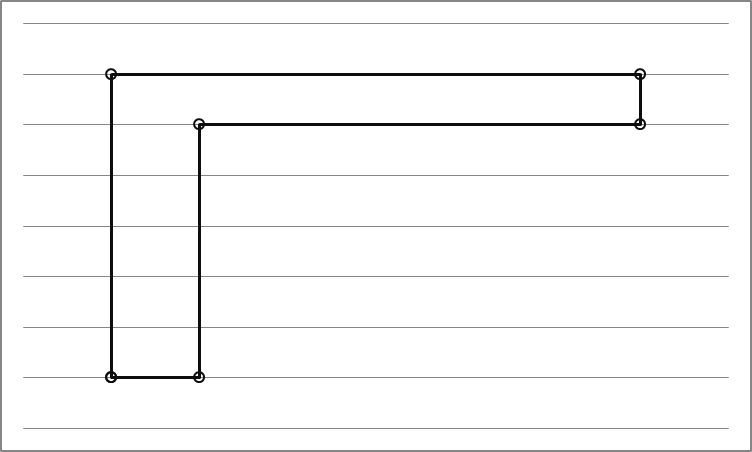
\includegraphics[width=\linewidth,keepaspectratio]{L}
\end{center}	
\end{frame}

%%%%%%%%%%%%%%%%%%%%%%%%%%%%%%%%%%%%%%%%%%%%%%%%%%%%%%%%%%%%%%%%%%%%%%%%%%%%%%%%%%
\begin{frame}[fragile]\frametitle{Few Shot Examples Shapes}
The last shape for which LLM has been asked for the answer is actually a ‘T’ shape. The picture below shows the correct/actual answer as well.

\begin{center}
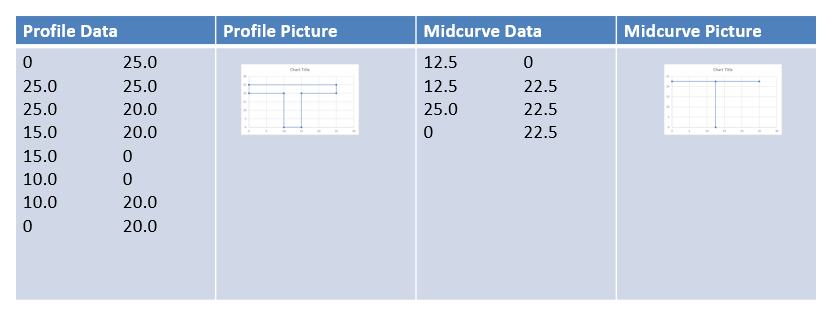
\includegraphics[width=\linewidth,keepaspectratio]{T}
\end{center}	
\end{frame}

%%%%%%%%%%%%%%%%%%%%%%%%%%%%%%%%%%%%%%%%%%%%%%%%%%%%%%%%%%%%%%%%%%%%%%%%%%%%%%%%%%
\begin{frame}[fragile]\frametitle{Output}
And the outputs computed by various LLMs (ChatGPT, Perplexity AI, Bard) , along with the real/actual answer:

\begin{lstlisting}
Actual: [((12.5,0), (12.5,22.5)), ((12.5,22.5),(25.0,22.5)), ((12.5,22.5),(0,22.5))]
ChatGPT: [((2.5, 0), (2.5, 22.5)), ((2.5, 22.5), (2.5, 45.0)), ((2.5, 22.5), (25.0, 22.5)), ((2.5, 22.5), (12.5, 22.5)), ((2.5, 22.5), (0, 22.5)), ((2.5, 22.5), (25.0, 22.5))]
Perplexity: [((12.5,0), (12.5, 22.5)), ((12.5, 22.5),(12.5,45.0)), ((12.5, 22.5), (0,22.5)), ((12.5, 22.5), (25.0,22.5))]
Bard: [((12.5, 0), (12.5, 25.0)), ((12.5, 25.0), (25.0, 25.0)), ((25.0, 25.0), (25.0, 0))]
\end{lstlisting}	
\end{frame}

%%%%%%%%%%%%%%%%%%%%%%%%%%%%%%%%%%%%%%%%%%%%%%%%%%%%%%%%%%%%%%%%%%%%%%%%%%%%%%%%%%
\begin{frame}[fragile]\frametitle{Output}

Visually here is how results from different LLMs look:

\begin{center}
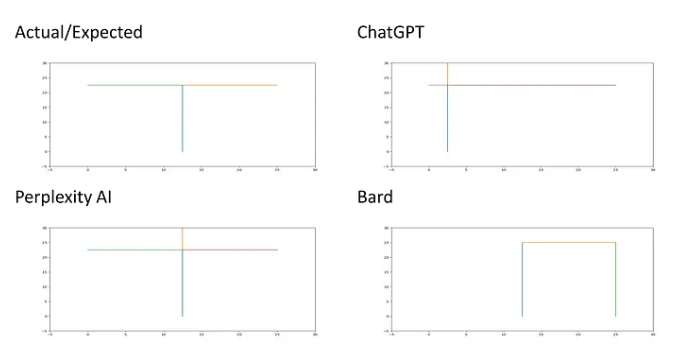
\includegraphics[width=\linewidth,keepaspectratio]{midcurve34}
\end{center}	
\end{frame}

%%%%%%%%%%%%%%%%%%%%%%%%%%%%%%%%%%%%%%%%%%%%%%%%%%%%%%%%%%%%%%%%%%%%%%%%%%%%%%%%%%
\begin{frame}[fragile]\frametitle{Interpretation}

All of the above have failed. Even latest (Oct 2023), the results are:
\begin{itemize}
\item \lstinline|llama 7B g4_0 ggml: (8, 17) & (64, 32): Wrong.|
\item \lstinline|Bard: [((8.33,5),(8.33, 22.5)), ((8.33, 22.5), (25,22.5)), ((8.33, 22.5), (0,25))]: Wrong.|
\item \lstinline|Hugging Chat: [((12.5, 0), (12.5, 22.5)), ((12.5, 22.5), (25.0, 22.5)), ((25.0, 22.5), (25.0, 25.0))]: a bit wrong on the last line|
\item \lstinline|GPT-4: [((12.5,0), (12.5,22.5)), ((12.5,22.5),(0,22.5)), ((12.5,22.5),(25.0,22.5))] just change in sequence of lines, and that's inconsequential, so the answer is correct.|
\end{itemize}	
\end{frame}

%%%%%%%%%%%%%%%%%%%%%%%%%%%%%%%%%%%%%%%%%%%%%%%%%%%%%%%%%%%%%%%%%%%%%%%%%%%%%%%%%%
\begin{frame}[fragile]\frametitle{Interpretation}

LLMs by an large seem to have failed for such simple shapes.

There could be two prominent reasons:

\begin{itemize}
\item The prompt design was not effective and could be improved upon.
\item The LLM model itself is not able to learn the pattern and predict well.
\end{itemize}	

The current geometry representation as a sequence of lines, has limitations. Trying to look for a good representation to store geometry/graph/network as text so that NLP (Natural Language Techniques) can be applied.
\end{frame}